% Two-stage retrieval. Each transformer layer runs both stages independently.
% Used in Chapter 3 (method) and referenced from Chapter 8 (walkthrough).

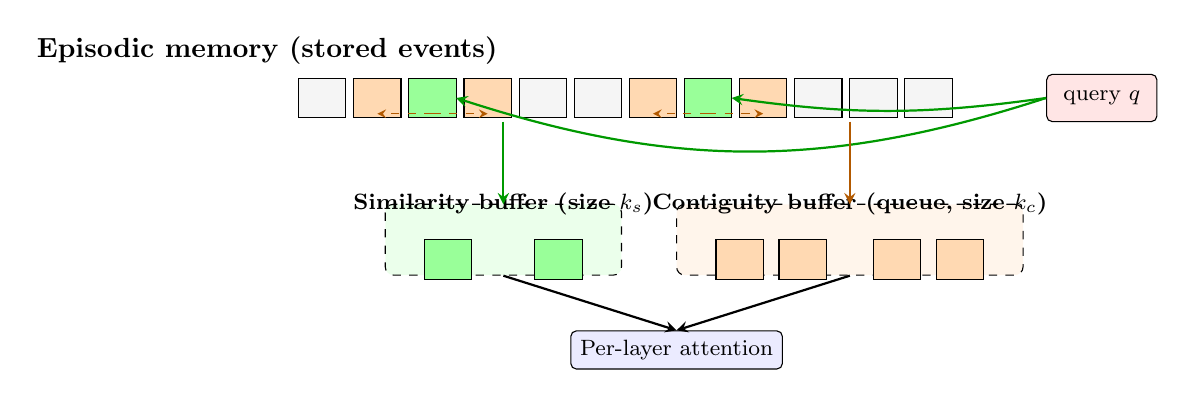
\begin{tikzpicture}[
  font=\footnotesize,
  event/.style={draw, rectangle, minimum width=0.6cm, minimum height=0.5cm, inner sep=1pt},
  query/.style={draw, rounded corners=2pt, fill=red!10, minimum width=1.4cm, minimum height=0.6cm},
  buffer/.style={draw, dashed, rounded corners=3pt, inner sep=6pt},
  arrow/.style={->, >=stealth, thick},
  faded/.style={fill=gray!8},
]

% Event store: a row of 12 stored events with two highlighted as top-k hits.
\node[font=\bfseries] at (0, 1.8) {Episodic memory (stored events)};
\foreach \i in {1,...,12} {
  \node[event, faded] (e\i) at (\i * 0.7, 1.2) {};
}
% Two top-similarity hits, dark green.
\node[event, fill=green!40] at (3 * 0.7, 1.2) {};
\node[event, fill=green!40] at (8 * 0.7, 1.2) {};
% Neighbours of the hits (enqueued into contiguity buffer), light orange.
\node[event, fill=orange!30] at (2 * 0.7, 1.2) {};
\node[event, fill=orange!30] at (4 * 0.7, 1.2) {};
\node[event, fill=orange!30] at (7 * 0.7, 1.2) {};
\node[event, fill=orange!30] at (9 * 0.7, 1.2) {};

% Query at the right.
\node[query] (q) at (10.6, 1.2) {query $q$};

% Similarity arrows (curved, green).
\draw[arrow, green!60!black] (q.west) to[bend left=18] (3 * 0.7 + 0.3, 1.2);
\draw[arrow, green!60!black] (q.west) to[bend left=8]  (8 * 0.7 + 0.3, 1.2);

% Contiguity arrows (curved, orange) from green hits to their neighbours.
\draw[->, >=stealth, dashed, orange!70!black] (3 * 0.7, 1.0) -- (2 * 0.7, 1.0);
\draw[->, >=stealth, dashed, orange!70!black] (3 * 0.7, 1.0) -- (4 * 0.7, 1.0);
\draw[->, >=stealth, dashed, orange!70!black] (8 * 0.7, 1.0) -- (7 * 0.7, 1.0);
\draw[->, >=stealth, dashed, orange!70!black] (8 * 0.7, 1.0) -- (9 * 0.7, 1.0);

% The two buffers below.
\node[buffer, fill=green!8, minimum width=3.0cm, minimum height=0.9cm] (simbuf) at (3.0, -0.6) {};
\node[font=\footnotesize\bfseries] at (3.0, -0.15) {Similarity buffer (size $k_s$)};
\node[event, fill=green!40] at (2.3, -0.85) {};
\node[event, fill=green!40] at (3.7, -0.85) {};

\node[buffer, fill=orange!8, minimum width=4.4cm, minimum height=0.9cm] (cbuf) at (7.4, -0.6) {};
\node[font=\footnotesize\bfseries] at (7.4, -0.15) {Contiguity buffer (queue, size $k_c$)};
\node[event, fill=orange!30] at (6.0, -0.85) {};
\node[event, fill=orange!30] at (6.8, -0.85) {};
\node[event, fill=orange!30] at (8.0, -0.85) {};
\node[event, fill=orange!30] at (8.8, -0.85) {};

% Arrows from the event store into the two buffers.
\draw[arrow, green!60!black] (3.0, 0.9) -- (3.0, -0.15);
\draw[arrow, orange!70!black] (7.4, 0.9) -- (7.4, -0.15);

% Final union arrow into attention.
\node[font=\footnotesize, draw, rounded corners=2pt, fill=blue!8, minimum width=2.4cm] (attn) at (5.2, -2.0) {Per-layer attention};
\draw[arrow] (simbuf.south) -- (attn.north);
\draw[arrow] (cbuf.south) -- (attn.north);

\end{tikzpicture}
